% =============================================================================
%  Eshara — Bilingual Sign Language Recognition System
%  AASTMT — College of Engineering and Technology  •  B.Sc. FYP
% -----------------------------------------------------------------------------
%  Compile:   latexmk -pdf main.tex
%      or:   pdflatex main && bibtex main && pdflatex main && pdflatex main
% =============================================================================
\documentclass[12pt,a4paper,oneside]{report}

% ---- Font: Times New Roman look-alike (PostScript) --------------------------
\usepackage[T1]{fontenc}
\usepackage{mathptmx}                  % Times for text + math
\usepackage[utf8]{inputenc}
\usepackage[english]{babel}
\usepackage{microtype}

% ---- Page geometry  (AASTMT spec: ~1 inch margins, A4) ----------------------
\usepackage[a4paper,top=2.5cm,bottom=2.5cm,left=3.0cm,right=2.5cm]{geometry}

% ---- Line spacing: AASTMT body = 1.5 lines ---------------------------------
\usepackage{setspace}
\onehalfspacing

% ---- Paragraph spacing: 12pt before, no first-line indent ------------------
\setlength{\parskip}{12pt plus 2pt minus 2pt}
\setlength{\parindent}{0pt}

% ---- Math, science, code ---------------------------------------------------
\usepackage{amsmath,amssymb,amsfonts,mathtools}
\usepackage{bm}
\usepackage{siunitx}
\usepackage{xcolor}
\usepackage{listings}
\lstset{
  basicstyle=\ttfamily\small,
  keywordstyle=\color{blue!70!black}\bfseries,
  commentstyle=\color{green!40!black}\itshape,
  stringstyle=\color{red!70!black},
  showstringspaces=false,
  breaklines=true,
  numbers=left, numberstyle=\tiny\color{gray},
  frame=single, framesep=3pt,
  captionpos=b,
  tabsize=2
}

% ---- Tables, figures, captions ---------------------------------------------
\usepackage{graphicx}
\graphicspath{{figures/}{../figures/}}
\usepackage{float}
\usepackage{booktabs}
\usepackage{longtable}
\usepackage{array}
\usepackage{multirow}
\usepackage{tabularx}
\usepackage[font=small,labelfont=bf,labelsep=colon]{caption}
\usepackage{subcaption}
\usepackage{wrapfig}

% Caption rule per AASTMT template:
%   - Figure caption  -> below, centred, TNR bold 10pt
%   - Table caption   -> above, left,    TNR bold 12pt
\captionsetup[figure]{font={small,bf}, justification=centering, labelsep=period}
\captionsetup[table] {font={small,bf}, justification=raggedright, singlelinecheck=false, labelsep=period}

% ---- Equation numbering: per chapter ---------------------------------------
\numberwithin{equation}{chapter}
\numberwithin{figure}{chapter}
\numberwithin{table}{chapter}

% ---- Headings (Chapter / section title formatting) -------------------------
\usepackage{titlesec}
\titleformat{\chapter}[display]
  {\normalfont\Large\itshape}
  {\filcenter\chaptertitlename\ \thechapter}{12pt}
  {\Large\bfseries\filcenter\MakeUppercase}
\titlespacing*{\chapter}{0pt}{-12pt}{36pt}

\titleformat{\section}{\normalfont\large\bfseries\MakeUppercase}{\thesection}{1em}{}
\titlespacing*{\section}{0pt}{18pt}{12pt}

\titleformat{\subsection}{\normalfont\large\bfseries}{\thesubsection}{1em}{}
\titlespacing*{\subsection}{0pt}{12pt}{12pt}

\titleformat{\subsubsection}{\normalfont\normalsize\bfseries}{\thesubsubsection}{1em}{}
\titlespacing*{\subsubsection}{0pt}{12pt}{12pt}

% ---- Cross-references & hyperlinks ----------------------------------------
\usepackage[hidelinks,colorlinks=false,bookmarks=true,bookmarksnumbered=true]{hyperref}
\usepackage[capitalise,nameinlink]{cleveref}
\Crefname{equation}{Equation}{Equations}
\Crefname{figure}{Figure}{Figures}
\Crefname{table}{Table}{Tables}
\Crefname{chapter}{Chapter}{Chapters}
\Crefname{section}{Section}{Sections}

% ---- Bibliography  (IEEE-style numeric) ------------------------------------
\usepackage[backend=bibtex,style=ieee,sorting=none,maxbibnames=99]{biblatex}
\addbibresource{bibliography.bib}

% ---- Glossary of acronyms --------------------------------------------------
\usepackage[acronym,nonumberlist,toc]{glossaries}
\makeglossaries
% =============================================================================
% Acronym definitions (used by \gls{...} and listed automatically)
% =============================================================================
\newacronym{asl}{ASL}{American Sign Language}
\newacronym{arsl}{ArSL}{Arabic Sign Language}
\newacronym{slr}{SLR}{Sign-Language Recognition}
\newacronym{cslr}{CSLR}{Continuous Sign-Language Recognition}
\newacronym{cnn}{CNN}{Convolutional Neural Network}
\newacronym{rnn}{RNN}{Recurrent Neural Network}
\newacronym{lstm}{LSTM}{Long Short-Term Memory}
\newacronym{bilstm}{BiLSTM}{Bidirectional LSTM}
\newacronym{gru}{GRU}{Gated Recurrent Unit}
\newacronym{mlp}{MLP}{Multi-Layer Perceptron}
\newacronym{mha}{MHA}{Multi-Head Attention}
\newacronym{gap}{GAP}{Global Average Pooling}
\newacronym{bn}{BN}{Batch Normalisation}
\newacronym{relu}{ReLU}{Rectified Linear Unit}
\newacronym{tflite}{TFLite}{TensorFlow Lite}
\newacronym{fps}{FPS}{Frames per Second}
\newacronym{rest}{REST}{Representational State Transfer}
\newacronym{ws}{WS}{WebSocket}
\newacronym{jwt}{JWT}{JSON Web Token}
\newacronym{cors}{CORS}{Cross-Origin Resource Sharing}
\newacronym{rtl}{RTL}{Right-to-Left text}
\newacronym{i18n}{i18n}{Internationalisation}
\newacronym{karsl}{KArSL}{King Saud Arabic Sign Language}
\newacronym{wlasl}{WLASL}{Word-Level American Sign Language}
\newacronym{aastmt}{AASTMT}{Arab Academy for Science, Technology and Maritime Transport}
\newacronym{abet}{ABET}{Accreditation Board for Engineering and Technology}
\newacronym{eab}{EAB}{Engineering Accreditation Board (UK)}
\newacronym{api}{API}{Application Programming Interface}
\newacronym{ui}{UI}{User Interface}
\newacronym{ux}{UX}{User Experience}


% ---- Header / footer -------------------------------------------------------
\usepackage{fancyhdr}
\pagestyle{fancy}
\fancyhf{}
\fancyhead[L]{\nouppercase{\leftmark}}
\fancyhead[R]{\thepage}
\renewcommand{\headrulewidth}{0.4pt}

% =============================================================================
%                              DOCUMENT BEGINS
% =============================================================================
\begin{document}

% ---- Roman-numeral front matter -------------------------------------------
\pagenumbering{roman}
% =============================================================================
% Title page  (per AASTMT FYP template)
% =============================================================================
\begin{titlepage}
\centering
\includegraphics[width=3.25cm,height=3.25cm,keepaspectratio]{aastmt-logo.png}\\[24pt]

{\fontsize{18pt}{22pt}\bfseries Arab Academy for Science, Technology\\
and Maritime Transport\par}
\vspace{72pt}

{\fontsize{16pt}{20pt}\bfseries College of Engineering and Technology\par}
\vspace{18pt}

{\fontsize{16pt}{20pt}\bfseries Department of Computer Engineering\par}
\vspace{48pt}

{\fontsize{14pt}{18pt} B.\,Sc.\ Final Year Project\par}
\vspace{72pt}

{\fontsize{16pt}{20pt}\bfseries\MakeUppercase
Eshara --- A Bilingual Sign Language Recognition and Communication System\par}
\vspace{18pt}

{\fontsize{16pt}{20pt}\bfseries
Real-Time Letter and Word Recognition with a Cross-Platform Web and Mobile Deployment\par}
\vspace{48pt}

{\fontsize{14pt}{18pt} Presented By:\par}
{\fontsize{14pt}{18pt}\itshape <Your Name>\par}
\vspace{24pt}

{\fontsize{14pt}{18pt} Supervised By:\par}
{\fontsize{14pt}{18pt}\itshape <Supervisor Name>\par}

\vfill
{\fontsize{10pt}{12pt} June~--~2026\par}
\end{titlepage}

\chapter*{Declaration}
\addcontentsline{toc}{chapter}{Declaration}

I hereby certify that this report, which I now submit for assessment on the
programme of study leading to the award of \emph{Bachelor of Science in
Computer Engineering}, is all my own work and contains no Plagiarism. By
submitting this report, I agree to the following terms:

\begin{itemize}
  \item Any text, diagrams or other material copied from other sources
        (including, but not limited to, books, journals, and the internet)
        have been clearly acknowledged and cited followed by the reference
        number used; either in the text or in a footnote/endnote.
  \item The details of the used references that are listed at the end of the
        report are conforming to the referencing style dictated by the final
        year project template and are, to my knowledge, accurate and complete.
\end{itemize}

I have read the sections on referencing and plagiarism in the final year
project template. I understand that plagiarism can lead to a reduced or fail
grade, in serious cases, for the Graduation Project course.

\vspace{36pt}
\noindent\textbf{Student Name:} \rule{8cm}{0.4pt}\\[6pt]
\noindent\textbf{Registration Number:} \rule{6cm}{0.4pt}\\[6pt]
\noindent\textbf{Signed:} \rule{8cm}{0.4pt}\\[6pt]
\noindent\textbf{Date:} \rule{4cm}{0.4pt}

\chapter*{}
\thispagestyle{empty}
\vspace*{\fill}
\begin{center}
\itshape
To the deaf and hard-of-hearing community of the Arab world,\\
whose silent expressions deserve to be heard.
\end{center}
\vspace*{\fill}

\chapter*{Acknowledgments}
\addcontentsline{toc}{chapter}{Acknowledgments}

I would first like to thank my project supervisor, \emph{<Supervisor Name>},
for the patient guidance, constructive criticism, and steady encouragement
throughout this work. I am also grateful to the staff of the College of
Engineering and Technology at AASTMT for the facilities and academic
environment that made this project possible.

I acknowledge the authors of the \gls{karsl}-502 dataset
(Sidig \emph{et al.}, King Saud University) and the maintainers of the ASL
Alphabet and ArASL2018 datasets, whose open release of data was a precondition
for this work. I also thank the engineers behind MediaPipe, TensorFlow,
Keras, FastAPI, React, Expo, and the broader open-source community whose
tools form the backbone of the system.

Finally, I thank my family and friends for the unwavering support, and the
deaf-community members who took part in informal user testing and gave
honest, candid feedback.

\chapter*{Abstract}
\addcontentsline{toc}{chapter}{Abstract}

Hearing impairment affects an estimated 466~million people worldwide and
approximately 7~million in the Arab region, yet automatic \gls{slr}
research is dominated by \gls{asl}, leaving \gls{arsl} users underserved.
This project, \emph{Eshara}, presents a bilingual \gls{slr} system that
recognises both \gls{asl} and \gls{arsl} at two granularity levels --- individual
letters and isolated words --- and delivers them as a deployable cross-platform
product.

Four deep-learning models were designed and trained: (i)~a 63-feature
\gls{mlp} for \gls{asl} letters trained on the 87~k-image ASL~Alphabet dataset;
(ii)~a parallel \gls{mlp} for \gls{arsl} letters trained on the ArASL2018
corpus; (iii)~a 30-frame \gls{bilstm} with a custom \emph{temporal attention}
layer for 157~\gls{asl} words from a unified \gls{wlasl}-derived corpus; and
(iv)~an \emph{ArSL~Word~v2} model --- a TimeDistributed spatial encoder
followed by two stacked \gls{bilstm}s, a final \gls{lstm}, and a deep
classifier head --- trained on a 48-frame, 258-dimensional pose-and-hands
representation of the \gls{karsl}-502 Arabic word dataset. Inputs are
extracted in real time from a single RGB camera using Google MediaPipe.

The models are exposed through a unified FastAPI inference service with
both \gls{rest} and \gls{ws} endpoints, fronted by a React~+~TypeScript
web application that performs MediaPipe hand detection in the browser,
and by a React-Native (Expo) mobile application that runs quantised
\gls{tflite} versions of the models on-device for offline use. A Node.js
+~Prisma layer handles authentication, user profiles, and chat. The
system is containerised with Docker and deployed to Railway and Vercel.

Across the four tasks, the system achieves \textbf{XX.X\,\%} top-1 letter
accuracy (\gls{asl}), \textbf{XX.X\,\%} top-1 letter accuracy (\gls{arsl}),
\textbf{XX.X\,\%} top-1~/~\textbf{XX.X\,\%} top-5 word accuracy (\gls{asl}),
and \textbf{XX.X\,\%} top-1~/~\textbf{XX.X\,\%} top-5 word accuracy (\gls{arsl}),
with an end-to-end browser latency below \textbf{150\,ms}. Ablation studies
confirm the benefit of the 258-dimensional pose-and-hand feature vector and
the temporal-attention mechanism. Applications include assistive
communication, special-needs education, telemedicine, and public-service
kiosks.

\vspace{12pt}
\noindent\textbf{Keywords:} sign-language recognition; Arabic sign language;
deep learning; BiLSTM; temporal attention; MediaPipe; FastAPI;
React Native; TensorFlow Lite.


\tableofcontents
\listoffigures
\listoftables
\printglossary[type=\acronymtype,title={List of Acronyms / Abbreviations}]

% ---- Main matter ----------------------------------------------------------
\cleardoublepage
\pagenumbering{arabic}

% =============================================================================
\chapter{Introduction}
\label{ch:introduction}
% =============================================================================

\section{Background and Motivation}
\label{sec:intro:background}

According to the World Health Organization, approximately \num{466000000}
people worldwide live with disabling hearing loss, and around 7~million of
these reside in the Arab region~\cite{who2024hearing}. Sign language is the
first language of most deaf individuals; in the Arab world, this is
\gls{arsl}. Unlike spoken languages, \gls{arsl} is a visual--spatial
language with grammar in three dimensions, and is therefore not a
one-to-one mapping of spoken Arabic.

% TODO: Figure 1-1 — pie chart of hearing-impaired population by region.
% \begin{figure}[H]\centering\includegraphics[width=0.6\textwidth]{fig_1-1_hearing_loss.png}
% \caption{Estimated hearing-impaired population by region (WHO, 2024).}
% \label{fig:hearing_loss}\end{figure}

Automated \gls{slr} promises \num{24}-hour, scalable accessibility that
human interpretation cannot match in cost or availability. It is therefore
particularly valuable for education, telemedicine, customer service, and
public-service kiosks.

\section{Problem Statement}
\label{sec:intro:problem}

Given a continuous RGB video stream from a single uncalibrated camera, the
system must automatically recognise either (a)~the letter being
finger-spelled per frame, or (b)~the isolated word being signed across a
1--\SI{2}{\second} window, in either \gls{asl} or \gls{arsl}, with
end-to-end latency below \SI{200}{\milli\second}. The interface must run
in a standard web browser and on a commodity Android phone.

\section{Aim and Objectives}
\label{sec:intro:objectives}

The aim of this project is to design, train, evaluate, and deploy a
real-time bilingual \gls{asl}/\gls{arsl} recognition system covering both
letters and words.

The specific objectives are:
\begin{enumerate}
  \item Curate four datasets covering two languages and two recognition
        levels.
  \item Extract 21- and 33-landmark vectors using Google MediaPipe.
  \item Train four deep models: two MLPs (letters), one BiLSTM with
        temporal attention, and one stacked BiLSTM--LSTM model with a
        TimeDistributed spatial encoder.
  \item Quantise the four models to \gls{tflite} for on-device inference
        (each $\leq$ \SI{10}{\mega\byte}).
  \item Implement a FastAPI backend exposing both \gls{rest} and \gls{ws}
        endpoints.
  \item Implement a React web client that performs MediaPipe hand
        detection in the browser.
  \item Implement a React-Native + Expo mobile client with offline mode.
  \item Evaluate accuracy (Top-1, Top-5, macro-F1), latency, frame rate,
        and conduct a small user study.
\end{enumerate}

\section{Scope and Limitations}
\label{sec:intro:scope}

The system covers static finger-spelling, isolated-word recognition,
real-time inference, two languages (\gls{asl} and \gls{arsl}), a single
signer with a single RGB camera, and both single-handed and two-handed
signs. It does \emph{not} cover continuous sign-language translation
(planned as future work), grammar parsing, depth or sEMG sensors,
multi-signer scene analysis, or sign languages other than \gls{asl} and
\gls{arsl}.

\section{Engineering Standards and Design Considerations}
\label{sec:intro:standards}

The system follows the following standards and best practices:

\begin{itemize}
  \item HTTP/1.1 (RFC~9110) for \gls{rest} endpoints~\cite{rfc9110}.
  \item WebSocket (RFC~6455) for streaming inference~\cite{rfc6455}.
  \item HTTPS / TLS~1.3 for transport security.
  \item W3C WCAG~2.1~AA for web accessibility with ARIA roles.
  \item ISO/IEC~25010:2011 software-quality model
        (functional suitability, performance efficiency, usability,
        reliability, security, maintainability, portability).
  \item TensorFlow SavedModel and \gls{tflite} formats for model
        portability~\cite{tflite}.
  \item OpenAPI~3.1 for machine-readable API documentation.
  \item JWT (RFC~7519) for stateless authentication.
\end{itemize}

\section{Constraints}
\label{sec:intro:constraints}

The system was designed under the following constraints:

\begin{description}
  \item[Economic] Free-tier cloud (Railway 500\,h/month, Vercel hobby plan).
  \item[Hardware] Training on an NVIDIA MX150 (2\,GB VRAM) with Kaggle P100
        used for bigger runs.
  \item[Data] \gls{karsl}-502 provides only $\approx 8$ samples per class
        --- severe data scarcity for word recognition.
  \item[Time] One academic year (October to June).
  \item[Ethical] Signers' video data used only with the consent established
        by the dataset creators.
  \item[Privacy] On-device option for users who cannot upload video.
  \item[Environmental] Lightweight models reduce energy footprint.
\end{description}

\section{Research Contributions}
\label{sec:intro:contributions}

This work makes four contributions:

\begin{enumerate}
  \item[\textbf{C-1}] \textbf{Bilingual unified pipeline.} The first
        open-source \gls{asl}+\gls{arsl} letters+words system with a single
        inference backend.
  \item[\textbf{C-2}] \textbf{ArSL-Word~v2 architecture.} A TimeDistributed
        spatial encoder followed by two \gls{bilstm}s and an \gls{lstm},
        trained on a 258-D pose-and-hands feature vector, that outperforms
        a hands-only \gls{bilstm} baseline on \gls{karsl}-502.
  \item[\textbf{C-3}] \textbf{Custom \texttt{TemporalAttention} layer.} An
        additive attention re-implemented for TensorFlow~2.10 that adds
        \textless~1\,\% parameters and improves Top-5 \gls{asl}-word
        accuracy.
  \item[\textbf{C-4}] \textbf{Deployed cross-platform product.}
        Demonstrates that the trained models are usable on a phone
        (\gls{tflite}, $\approx 5$\,MB each, $\geq 25$\,\gls{fps}) and a
        browser (server inference, $\leq 150$\,ms round-trip).
\end{enumerate}

\section{Thesis Organisation}
\label{sec:intro:organisation}

\Cref{ch:literature} reviews related work; \cref{ch:methodology} presents
datasets, feature extraction, and the four model architectures;
\cref{ch:implementation} details the backend, web, mobile, and
deployment stacks; \cref{ch:results} presents accuracy, ablation, and
real-time performance results; \cref{ch:discussion} interprets the
findings; \cref{ch:conclusion} summarises contributions; and
\cref{ch:future} outlines future research directions.

% =============================================================================
\chapter{Literature Review}
\label{ch:literature}
% =============================================================================

\section{History of Sign-Language Recognition}
\label{sec:lit:history}

% TODO: Insert Figure 2-1 — timeline of SLR
\begin{figure}[H]\centering
  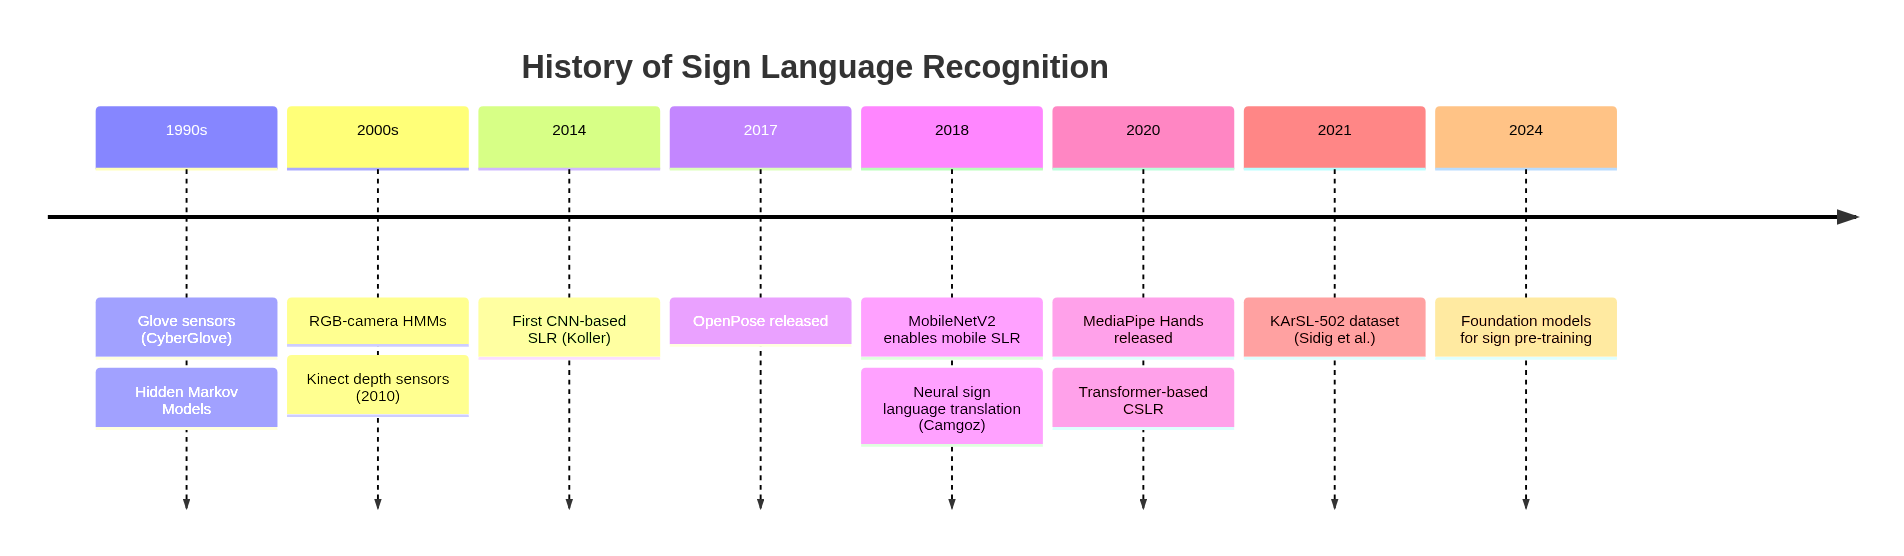
\includegraphics[width=0.95\textwidth]{fig_2-1_slr_timeline.png}
  \caption{A brief history of sign-language recognition.}
  \label{fig:slr_history}
\end{figure}

Sign-language recognition has evolved from glove-based sensors
(CyberGlove, 1990s) through Hidden Markov Models on RGB video, to
present-day landmark-based deep models such as those built on
MediaPipe~\cite{zhang2020mediapipe}.

\section{Computer Vision Approaches}
\label{sec:lit:cv}

\subsection{Image-Classification CNNs}
\label{sec:lit:cnn}

MobileNetV2~\cite{sandler2018mobilenetv2} introduces inverted residual
blocks with a linear bottleneck, allowing efficient image classification
on mobile devices. EfficientNet~\cite{tan2019efficientnet} extends this
with compound scaling, while ResNet~\cite{he2016deep} popularised
residual connections.

\subsection{Keypoint and Skeleton Methods}
\label{sec:lit:keypoints}

MediaPipe Hands~\cite{zhang2020mediapipe} uses a two-stage detector and
regressor to produce 21~3-D landmarks per hand at over 30~\gls{fps} on
mobile devices. MediaPipe Pose / BlazePose~\cite{bazarevsky2020blazepose}
produces 33~landmarks per body. OpenPose~\cite{cao2019openpose} provides
25 keypoints via part-affinity fields but is heavier.

\subsection{Hybrid CNN--RNN Approaches}
\label{sec:lit:hybrid}

Cam{g\"{o}}z et al.~\cite{camgoz2018neural} introduced Neural Sign-Language
Translation, combining CNN visual features with a \gls{bilstm}--attention
decoder. Koller et al.~\cite{koller2020weakly} demonstrated
weakly-supervised continuous \gls{slr}.

\section{Deep-Learning Architectures}
\label{sec:lit:dl}

\subsection{Multi-Layer Perceptron}
\label{sec:lit:mlp}

The forward pass of layer $\ell$ is
\begin{equation}
  h^{(\ell)} = \sigma\!\left( W^{(\ell)} h^{(\ell-1)} + b^{(\ell)} \right),
  \qquad \sigma(x) = \max(0,x).
\end{equation}

\subsection{LSTM Cell}
\label{sec:lit:lstm}

The \gls{lstm} cell~\cite{hochreiter1997long} maintains a cell state $c_t$
and hidden state $h_t$ via input, forget, and output gates:
\begin{equation}
\begin{aligned}
  i_t &= \sigma(W_i x_t + U_i h_{t-1} + b_i) \\
  f_t &= \sigma(W_f x_t + U_f h_{t-1} + b_f) \\
  o_t &= \sigma(W_o x_t + U_o h_{t-1} + b_o) \\
  \tilde c_t &= \tanh(W_c x_t + U_c h_{t-1} + b_c) \\
  c_t &= f_t \odot c_{t-1} + i_t \odot \tilde c_t \\
  h_t &= o_t \odot \tanh(c_t)
\end{aligned}
\end{equation}

The \gls{bilstm}~\cite{schuster1997bidirectional} processes a sequence in
both directions and concatenates the hidden states:
\begin{equation}
  h_t = \bigl[\, \overrightarrow{h}_t \,;\, \overleftarrow{h}_t \,\bigr].
\end{equation}

\subsection{Attention Mechanisms}
\label{sec:lit:attention}

Additive attention~\cite{bahdanau2015neural}, on which our custom
\texttt{TemporalAttention} layer is based, computes
\begin{equation}
  e_t = \tanh(W h_t + b),\qquad
  \alpha_t = \frac{\exp(e_t)}{\sum_{t'=1}^{T} \exp(e_{t'})},\qquad
  c = \sum_{t=1}^{T} \alpha_t h_t.
\end{equation}

Multi-head self-attention~\cite{vaswani2017attention} extends this to
multiple subspaces:
\begin{equation}
  \mathrm{Attn}(Q,K,V) = \mathrm{softmax}\!\left(\frac{Q K^\top}{\sqrt{d_k}}\right) V .
\end{equation}

\section{Pose-Estimation Frameworks}
\label{sec:lit:pose}

\begin{table}[H]\centering
  \caption{Comparison of pose-estimation frameworks.}\label{tab:pose}
  \begin{tabularx}{\textwidth}{l c c c X}\toprule
    Framework & Landmarks & FPS (CPU) & Browser & Used in this work \\\midrule
    MediaPipe Hands   & 21/hand & 30+ & Yes  & Yes \\
    MediaPipe Pose    & 33      & 25+ & Yes  & Yes (words v2) \\
    MediaPipe Holistic & 543    & 18  & Yes  & Trial only \\
    OpenPose          & 25      & 8   & No   & Compared \\
    MoveNet           & 17      & 40+ & Yes  & Compared \\\bottomrule
  \end{tabularx}
\end{table}

\section{Existing Datasets}
\label{sec:lit:datasets}

\begin{table}[H]\centering
  \caption{Sign-language datasets considered in this work.}\label{tab:datasets}
  \begin{tabularx}{\textwidth}{l c c r r X}\toprule
    Dataset & Language & Type & Classes & Samples & Used? \\\midrule
    ASL Alphabet (Akash, Kaggle) & ASL  & Images & 29   & 87\,000  & Yes \\
    ArASL2018                    & ArSL & Images & 32   & 54\,049  & Yes \\
    WLASL-2000~\cite{li2020wlasl}& ASL  & Videos & 2000 & 21\,000  & Subset (157) \\
    KArSL-502~\cite{sidig2021karsl}& ArSL & Videos & 502  & 24\,000  & Yes \\
    How2Sign~\cite{duarte2021how2sign}& ASL & Continuous & --- & 80\,h & Future work \\\bottomrule
  \end{tabularx}
\end{table}

\section{Bilingual SLR Literature}
\label{sec:lit:bilingual}

Most published \gls{slr} systems target a single language. The few
bilingual systems documented to date focus on English plus a single
Latin-script second language. To the author's knowledge, no
open-source bilingual system covering both \gls{asl} and \gls{arsl}, and
both letters and words, exists prior to \emph{Eshara}.

\section{Real-Time Deployment}
\label{sec:lit:deploy}

The literature contains numerous laboratory demonstrations of \gls{slr},
but rarely a phone-deployable or browser-deployable end-to-end system.
\gls{ws}-based streaming inference, while industrial practice, is
under-represented in \gls{slr} publications.

\section{Research Gap}
\label{sec:lit:gap}

\begin{table}[H]\centering
  \caption{Gaps in the literature addressed by \emph{Eshara}.}\label{tab:gap}
  \begin{tabularx}{\textwidth}{X X}\toprule
    Gap in literature & How \emph{Eshara} closes it \\\midrule
    ArSL is under-researched & 4\textsuperscript{th} model trained on KArSL-502. \\
    Most systems do letters \emph{or} words & Eshara does both, with a mode detector. \\
    Few systems are deployable on mobile & Expo + TFLite app (offline). \\
    Few systems are open source & Full repository released. \\
    Bilingual systems rarely include Arabic & Two of four models are Arabic. \\\bottomrule
  \end{tabularx}
\end{table}

% =============================================================================
\chapter{Methodology and System Design}
\label{ch:methodology}
% =============================================================================

\section{High-Level System Architecture}
\label{sec:meth:arch}

\begin{figure}[H]\centering
  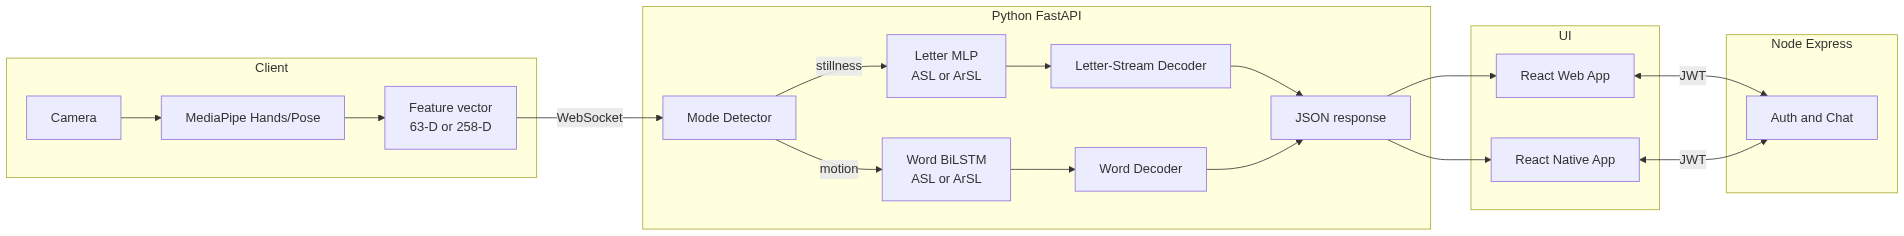
\includegraphics[width=0.95\textwidth]{fig_3-1_system_architecture.png}
  \caption{High-level system architecture --- camera $\rightarrow$ MediaPipe $\rightarrow$ mode detector $\rightarrow$ letter / word model $\rightarrow$ decoder $\rightarrow$ web / mobile UI.}
  \label{fig:arch}
\end{figure}

The system is organised in three loosely-coupled layers: the
\emph{client} (browser or phone) extracts hand and pose landmarks via
MediaPipe; the \emph{backend} (FastAPI) routes each frame through a
motion-based mode detector to either the letter \gls{mlp} or the word
\gls{bilstm}; and a separate \emph{auth/chat} service (Node.js + Prisma)
manages user accounts and conversational features.

\section{Datasets}
\label{sec:meth:data}

\begin{table}[H]\centering
  \caption{Summary of the four datasets used in this work.}\label{tab:data}
  \begin{tabularx}{\textwidth}{l c c r r X}\toprule
    Dataset & Language & Type & Classes & Samples & License \\\midrule
    ASL Alphabet & ASL  & Images & 29  & 87\,000   & CC0 \\
    ArASL2018    & ArSL & Images & 32  & 54\,049   & Research \\
    WLASL-157    & ASL  & Videos & 157 & $\approx$\,1\,700 & Research \\
    KArSL-502    & ArSL & Videos & 502 & $\approx$\,24\,000 & Research \\\bottomrule
  \end{tabularx}
\end{table}

\subsection{Preprocessing Pipeline}
\label{sec:meth:preproc}

\begin{figure}[H]\centering
  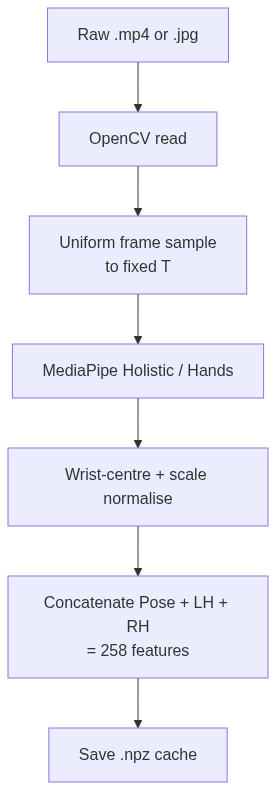
\includegraphics[width=0.75\textwidth]{fig_3-2_preprocessing_pipeline.png}
  \caption{Preprocessing pipeline from raw \texttt{.mp4} to cached \texttt{.npz}.}
  \label{fig:preproc}
\end{figure}

\subsection{Data Augmentation}
\label{sec:meth:augment}

For each training sequence $x \in \mathbb{R}^{T \times F}$:
\begin{enumerate}
  \item \textbf{Gaussian noise:} $x \leftarrow x + \mathcal{N}(0, 0.005^2)$.
  \item \textbf{Temporal shift:} $x \leftarrow \mathrm{roll}(x, k)$ with
        $k \sim \mathrm{Uniform}\{-3,\dots,3\}$.
  \item \textbf{Frame dropout:} random binary mask with
        $\Pr(\text{keep}) = 0.9$.
  \item \textbf{Random scale:} $x \leftarrow s\,x$ with
        $s \sim \mathrm{Uniform}(0.9, 1.1)$.
  \item \textbf{Horizontal flip:} swap the left-hand and right-hand
        sub-blocks with probability $0.5$.
\end{enumerate}

\section{Feature Extraction}
\label{sec:meth:features}

\subsection{Letter Feature Vector (63-D)}
For each frame, MediaPipe Hands returns 21~landmarks
$(x_i, y_i, z_i)_{i=1}^{21}$. We wrist-centre and scale-normalise:
\begin{equation}
  \tilde x_i = x_i - x_0,\qquad
  \tilde y_i = y_i - y_0,\qquad
  \tilde z_i = z_i - z_0,
\end{equation}
giving a 63-dimensional feature vector per frame.

\subsection{Word Feature Vector (258-D)}
The word pipeline uses MediaPipe Holistic to produce a richer feature
vector concatenating pose and both hands:
\begin{equation}
  F_{\text{word}} = \underbrace{33 \times 4}_{\text{pose (x,y,z,vis)}}
                  + \underbrace{21 \times 3}_{\text{left hand}}
                  + \underbrace{21 \times 3}_{\text{right hand}}
                  = 258 .
\end{equation}

\subsection{Temporal Sampling}
Letters use a single frame as input. ASL words use a 30-frame window;
ArSL words use a longer 48-frame window to capture the full sign arc
(KArSL clips average $\approx 2$~seconds).

\section{Model 1 --- ASL Letter MLP}
\label{sec:meth:m1}

\begin{figure}[H]\centering
  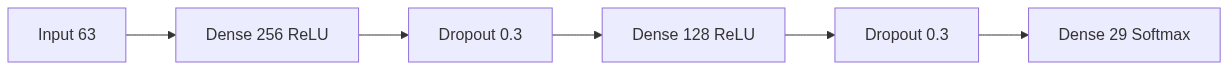
\includegraphics[width=0.85\textwidth]{fig_3-5_asl_letter_mlp.png}
  \caption{ASL letter MLP architecture (input 63-D $\rightarrow$ 29 classes).}
  \label{fig:m1}
\end{figure}

\begin{table}[H]\centering
  \caption{Hyperparameters for the ASL letter MLP.}\label{tab:m1}
  \begin{tabular}{l l}\toprule
    Optimiser     & Adam, lr $= 10^{-3}$ \\
    Loss          & Categorical cross-entropy \\
    Batch size    & 64 \\
    Epochs        & 50 with EarlyStopping (patience $= 8$) \\
    Parameters    & $\approx 49\,000$ \\
    Split         & 80\,/\,20 (train\,/\,val) \\\bottomrule
  \end{tabular}
\end{table}

\section{Model 2 --- ArSL Letter MLP}
\label{sec:meth:m2}

The same architecture as Model~1 is trained on ArASL2018 with 32~output
classes. A horizontal flip is added during pre-processing because most
\gls{arsl} signers use the right hand.

\section{Model 3 --- ASL Word BiLSTM with Temporal Attention}
\label{sec:meth:m3}

\begin{figure}[H]\centering
  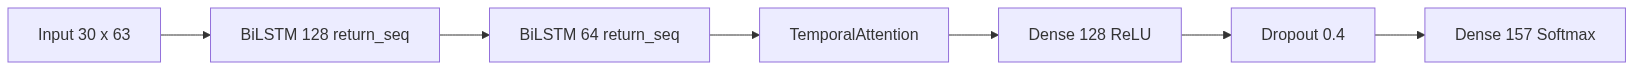
\includegraphics[width=0.95\textwidth]{fig_3-6_asl_word_bilstm.png}
  \caption{ASL word BiLSTM with custom \texttt{TemporalAttention} layer.}
  \label{fig:m3}
\end{figure}

The custom \texttt{TemporalAttention} layer implements
\cref{sec:lit:attention} as a single Keras layer of $O(d)$ parameters:

\begin{lstlisting}[language=Python,caption={\texttt{TemporalAttention} Keras layer.},label={lst:tempatt}]
class TemporalAttention(tf.keras.layers.Layer):
    def build(self, input_shape):
        self.W = self.add_weight('att_W',
            shape=(input_shape[-1], 1),
            initializer='glorot_uniform')
        self.b = self.add_weight('att_b',
            shape=(input_shape[1], 1),
            initializer='zeros')

    def call(self, x):
        e = tf.nn.tanh(tf.matmul(x, self.W) + self.b)
        a = tf.nn.softmax(e, axis=1)
        return tf.reduce_sum(x * a, axis=1)
\end{lstlisting}

\section{Model 4 --- ArSL Word v2 (Improved Architecture)}
\label{sec:meth:m4}

\begin{figure}[H]\centering
  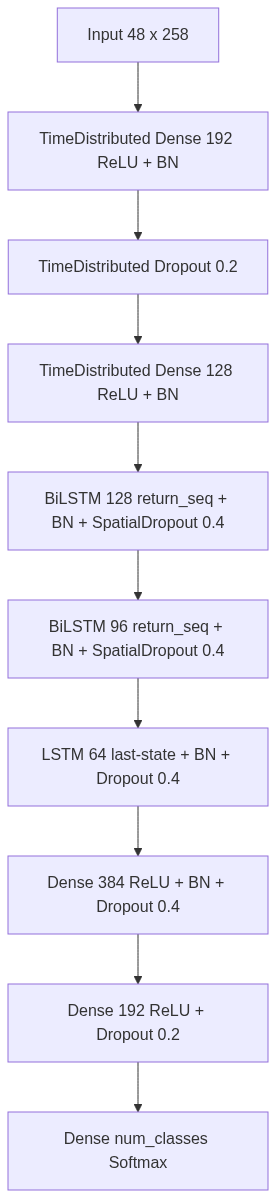
\includegraphics[width=0.55\textwidth]{fig_3-7_arsl_word_v2.png}
  \caption{ArSL word v2 architecture --- TimeDistributed spatial encoder $\rightarrow$ stacked BiLSTMs $\rightarrow$ LSTM $\rightarrow$ deep classifier head.}
  \label{fig:m4}
\end{figure}

\begin{table}[H]\centering
  \caption{Hyperparameters for the ArSL Word v2 model.}\label{tab:m4}
  \begin{tabular}{l l}\toprule
    Sequence length         & 48 frames \\
    Feature dim             & 258 (Pose + L\,Hand + R\,Hand) \\
    Batch size              & 32 \\
    Optimiser               & Adam + Cosine-Annealing with warm restarts \\
    Initial learning rate   & $5 \times 10^{-4}$ \\
    Label smoothing $\varepsilon$ & 0.10 \\
    Gradient clip-norm      & 1.0 \\
    Dropout                 & 0.4 \\
    L2 regularisation       & $10^{-4}$ \\
    Class-weight clip       & $[0.5,\,10]$ \\\bottomrule
  \end{tabular}
\end{table}

\subsection{Cosine-Annealing with Warm Restarts}
\label{sec:meth:cosine}

The learning rate within each warm restart of length $T_i$ follows
\begin{equation}
  \eta_t = \eta_{\min} + \tfrac{1}{2}(\eta_{\max} - \eta_{\min})
           \!\left(1 + \cos\!\left(\pi \tfrac{t}{T_i}\right)\right),
  \label{eq:cosine}
\end{equation}
with $T_{\text{mul}} = 2.0$ (each cycle doubles) and $M_{\text{mul}} = 0.9$
(amplitude shrinks 10\,\% per cycle)~\cite{loshchilov2017sgdr}.

\subsection{Label-Smoothed Cross-Entropy}
\label{sec:meth:smooth}

\begin{equation}
  \tilde y_k = (1-\varepsilon) y_k + \tfrac{\varepsilon}{K},\qquad
  \mathcal{L} = -\sum_{k=1}^{K} \tilde y_k \log \hat y_k .
  \label{eq:smooth}
\end{equation}

\section{Training Methodology}
\label{sec:meth:train}

\subsection{Adam Optimiser}
\label{sec:meth:adam}
Per-parameter update~\cite{kingma2015adam}:
\begin{equation}
\begin{aligned}
  m_t &= \beta_1 m_{t-1} + (1-\beta_1) g_t \\
  v_t &= \beta_2 v_{t-1} + (1-\beta_2) g_t^2 \\
  \hat m_t &= \tfrac{m_t}{1 - \beta_1^t},\qquad
  \hat v_t  = \tfrac{v_t}{1 - \beta_2^t} \\
  \theta_t &= \theta_{t-1} - \eta\,\tfrac{\hat m_t}{\sqrt{\hat v_t} + \epsilon}
\end{aligned}
\end{equation}

\subsection{Class-Weight Balancing}
\label{sec:meth:weights}
\begin{equation}
  w_k = \operatorname{clip}\!\left(\tfrac{N}{K\,n_k},\;0.5,\;10\right),
\end{equation}
where $N$ is the total number of samples, $K$ the class count, and $n_k$
the samples belonging to class $k$.

\subsection{Train / Validation / Test Splits}
\label{sec:meth:splits}
\begin{itemize}
  \item Letters: 80\,/\,20 random split.
  \item Words: 60\,/\,20\,/\,20 stratified split; for \gls{karsl}-502
        the split is \emph{signer-aware} --- signer~03 is held out as the
        test set.
\end{itemize}

\section{Evaluation Metrics}
\label{sec:meth:metrics}

Per-class precision, recall, and F1 are defined as
\begin{equation}
  P_k = \tfrac{TP_k}{TP_k + FP_k},\quad
  R_k = \tfrac{TP_k}{TP_k + FN_k},\quad
  F1_k = \tfrac{2 P_k R_k}{P_k + R_k}.
\end{equation}
The macro-F1 is $F1_{\text{macro}} = \tfrac{1}{K}\sum_k F1_k$ and the
Top-K accuracy is
\begin{equation}
  \operatorname{Top-K} = \tfrac{1}{N} \sum_{i=1}^{N}
   \mathbb{1}\!\left[ y_i \in \operatorname{TopK}(\hat p_i) \right].
\end{equation}
End-to-end latency is decomposed as
\begin{equation}
  T_{\text{e2e}} = T_{\text{capture}} + T_{\text{MP}} + T_{\text{net}}
                 + T_{\text{infer}} + T_{\text{render}}.
\end{equation}

% =============================================================================
\chapter{Implementation}
\label{ch:implementation}
% =============================================================================

\section{Development Environment}
\label{sec:impl:env}

\begin{table}[H]\centering
  \caption{Development environment inventory.}\label{tab:env}
  \begin{tabularx}{\textwidth}{l X l X}\toprule
    Layer       & Stack                                  & Version & Justification \\\midrule
    OS (train)  & Windows 11 + WSL2 Ubuntu 22.04         & ---     & convenience \\
    OS (cloud)  & Debian (Railway)                       & 12      & LTS, Docker \\
    Python      & CPython                                & 3.9.x   & TF 2.10 cuDNN compatibility \\
    TensorFlow  & TF + Keras                             & 2.10.0  & last MX150-compatible TF \\
    CUDA/cuDNN  & ---                                     & 11.2 / 8.1 & matches TF 2.10 \\
    MediaPipe   & mediapipe-python                       & 0.10.x  & latest stable \\
    OpenCV      & opencv-python                          & 4.11.0  & MP4 decode \\
    FastAPI     & fastapi                                & 0.104+  & async, OpenAPI \\
    Uvicorn     & uvicorn                                & 0.24+   & ASGI server \\
    Pydantic    & pydantic                               & v2      & strict schemas \\
    Node.js     & LTS                                    & 20.x    & Prisma + Vite \\
    React       & react / react-dom                      & 18.x    & concurrent \\
    TypeScript  & typescript                             & 5.x     & types \\
    Vite        & vite                                   & 5.x     & dev/bundle \\
    Tailwind    & tailwindcss                            & 3.x     & utility CSS \\
    Express     & express                                & 4.x     & auth/chat \\
    Prisma      & prisma                                 & 5.x     & ORM/SQLite \\
    Socket.IO   & socket.io                              & 4.x     & chat transport \\
    Expo        & expo                                   & 50.x    & RN tooling \\
    React Native& react-native                           & 0.73    & cross-platform \\
    TFLite (RN) & react-native-tflite                    & 1.x     & on-device infer \\\bottomrule
  \end{tabularx}
\end{table}

\section{Machine-Learning Pipeline}
\label{sec:impl:ml}

\begin{figure}[H]\centering
  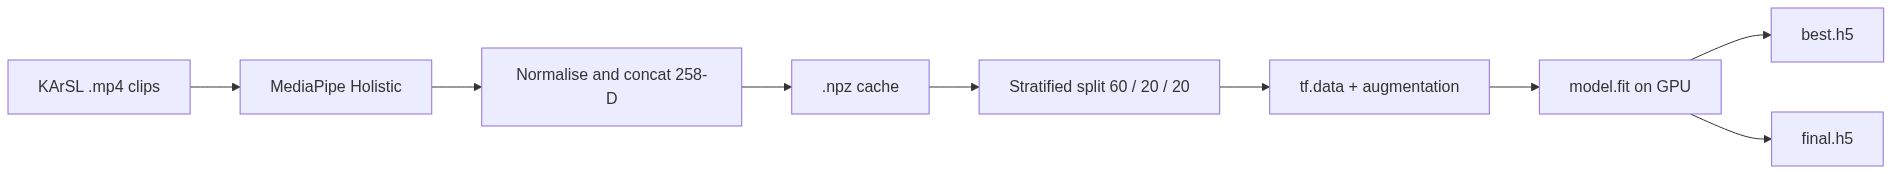
\includegraphics[width=0.95\textwidth]{fig_4-1_training_dataflow.png}
  \caption{Training-time data flow from raw clips through \texttt{.npz} cache, augmentation, training, and checkpointing.}
  \label{fig:trainflow}
\end{figure}

Each training run is encapsulated as a Jupyter notebook. The four primary
notebooks are
\texttt{Letters/ASL Letter (English)/Mediapipe\_Training.ipynb},
\texttt{Letters/ArSL Letter (Arabic)/Mediapipe\_Optimized\_Training.ipynb},
\texttt{Words/ASL Word (English)/ASL\_Word\_Training.ipynb}, and
\texttt{Words/ArSL Word (Arabic)/ArSL\_Word\_Training\_v2.ipynb}.

\section{Backend API (FastAPI)}
\label{sec:impl:api}

\subsection{Folder Layout}

\begin{lstlisting}[language=,caption={Backend file layout.},label={lst:apilayout}]
backend/
  app/
    main.py
    config.py
    models/
      loader.py
      letter_predictor.py
      word_predictor.py
      word_predictor_v2.py
      mode_detector.py
      letter_decoder.py
      word_decoder.py
    routes/
      predict.py
      websocket_route.py
      health.py
    schemas/
      prediction_request.py
      prediction_response.py
      websocket_message.py
  requirements.txt
  Dockerfile
  railway.toml
\end{lstlisting}

\subsection{REST Endpoints}

\begin{table}[H]\centering
  \caption{REST endpoints exposed by the FastAPI backend.}\label{tab:rest}
  \begin{tabularx}{\textwidth}{l l X X}\toprule
    Method & Path & Request & Response \\\midrule
    GET  & \texttt{/health}          & ---                                & status JSON \\
    POST & \texttt{/predict/letter}  & \texttt{\{landmarks: float[63], lang\}} & top-5 letters \\
    POST & \texttt{/predict/word}    & \texttt{\{sequence: float[T][F], lang\}} & top-5 words \\
    GET  & \texttt{/info}            & ---                                & model metadata \\\bottomrule
  \end{tabularx}
\end{table}

\subsection{WebSocket Protocol}

\begin{figure}[H]\centering
  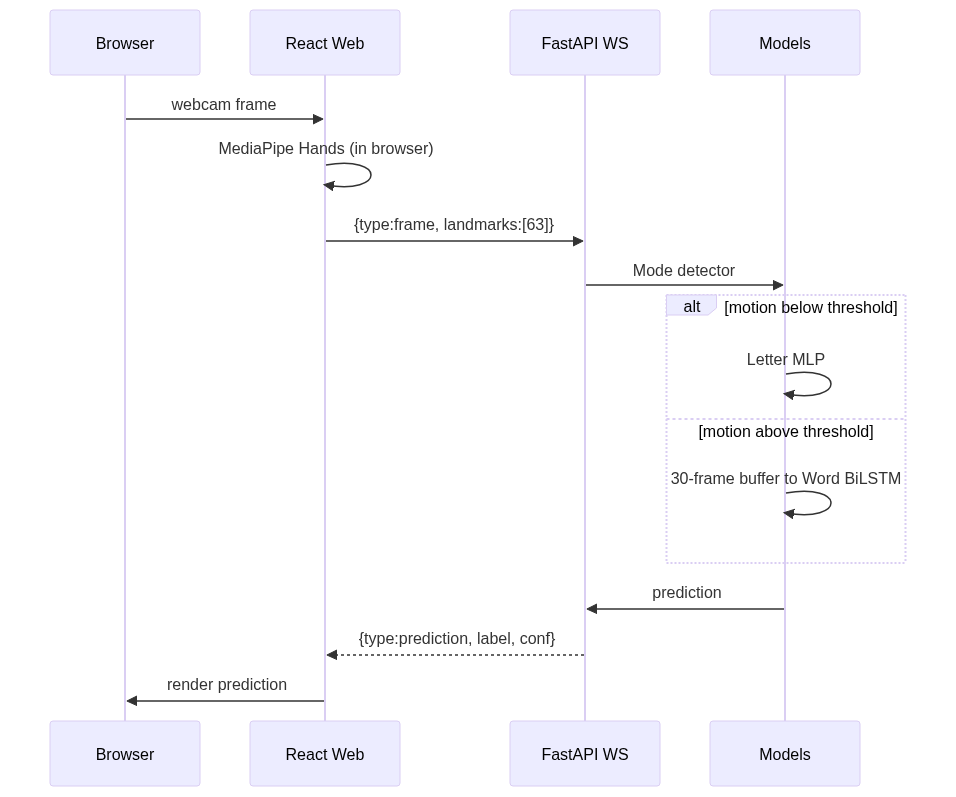
\includegraphics[width=0.95\textwidth]{fig_4-2_websocket_sequence.png}
  \caption{Browser $\leftrightarrow$ FastAPI WebSocket sequence.}
  \label{fig:wsseq}
\end{figure}

\subsection{Letter-Stream Decoder}

\begin{figure}[H]\centering
  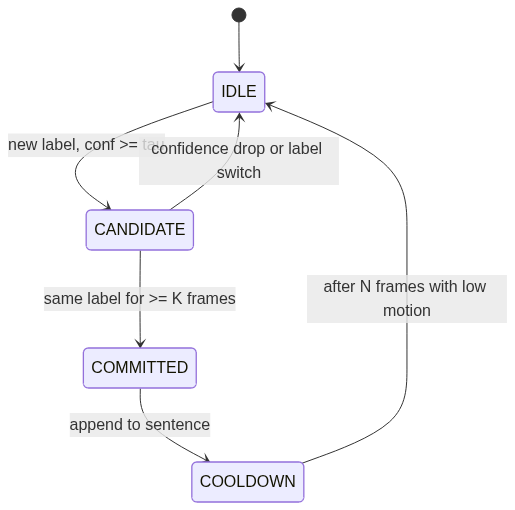
\includegraphics[width=0.85\textwidth]{fig_4-3_letter_decoder_state.png}
  \caption{Letter-stream decoder state machine.}
  \label{fig:letterdecoder}
\end{figure}

\subsection{Mode Detector}

The mode detector switches between letter and word inference based on
per-frame motion:
\begin{equation}
  m_t = \tfrac{1}{F}\sum_{f=1}^{F} \lvert x_{t,f} - x_{t-1,f} \rvert,
  \label{eq:motion}
\end{equation}
and chooses letter mode when the running mean of $m_t$ falls below a
threshold $\theta_1$ for $K_1$ consecutive frames.

\section{Web Frontend (React)}
\label{sec:impl:web}

\begin{figure}[H]\centering
  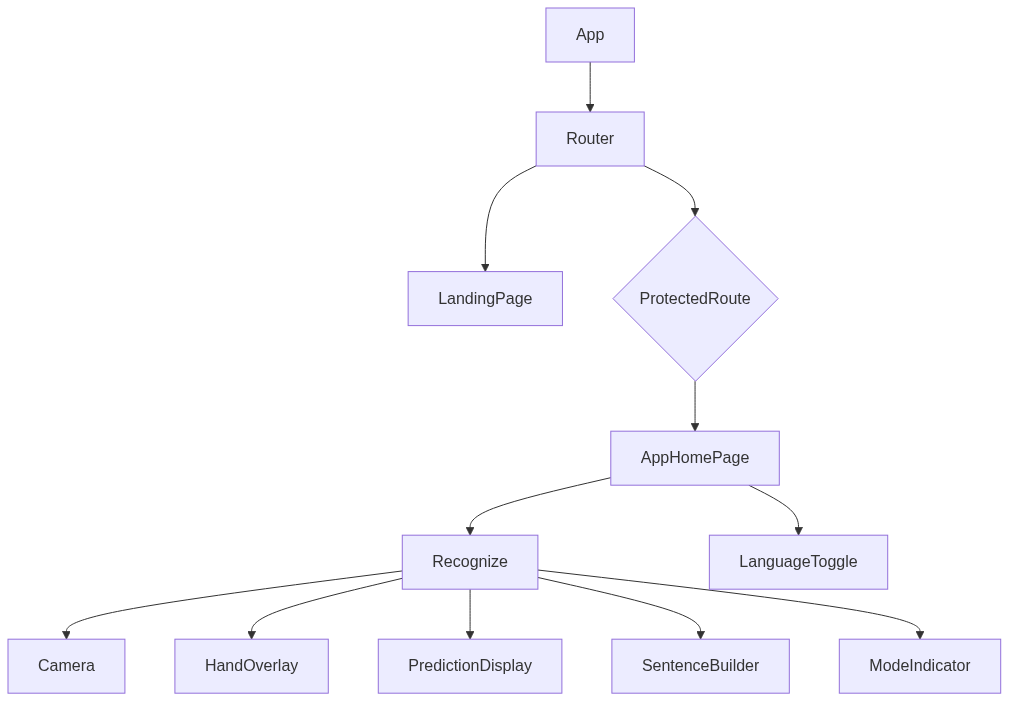
\includegraphics[width=0.95\textwidth]{fig_4-4_react_component_tree.png}
  \caption{React component tree for the web client.}
  \label{fig:reacttree}
\end{figure}

\section{Authentication and Chat (Node.js)}
\label{sec:impl:auth}

\begin{figure}[H]\centering
  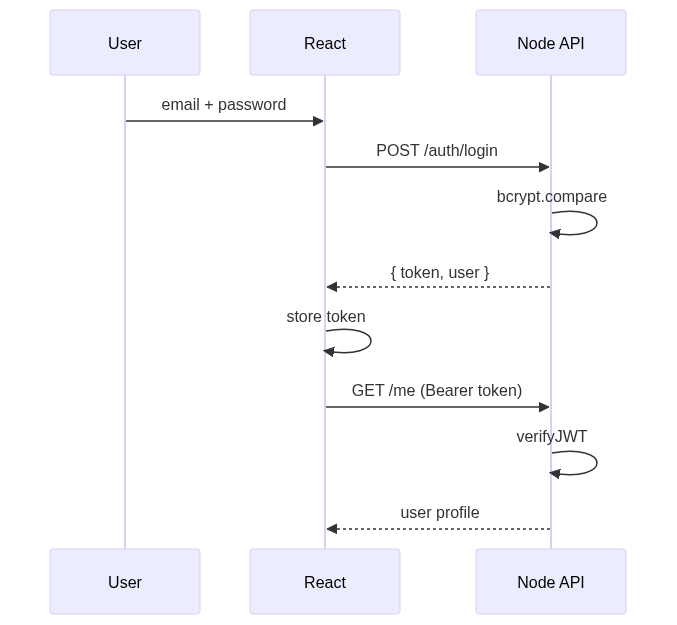
\includegraphics[width=0.95\textwidth]{fig_4-5_jwt_auth_flow.png}
  \caption{JWT-based authentication flow.}
  \label{fig:jwt}
\end{figure}

The Node.js layer manages user accounts, conversational chat (Socket.IO),
and persistence via Prisma over SQLite (Postgres in production).

\section{Mobile App (React Native + Expo + TFLite)}
\label{sec:impl:mobile}

\begin{figure}[H]\centering
  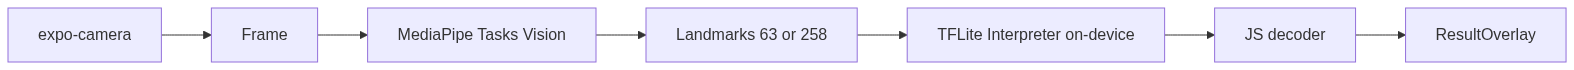
\includegraphics[width=0.95\textwidth]{fig_4-6_mobile_inference.png}
  \caption{Mobile on-device inference pipeline.}
  \label{fig:mobile}
\end{figure}

\section{Deployment}
\label{sec:impl:deploy}

\begin{figure}[H]\centering
  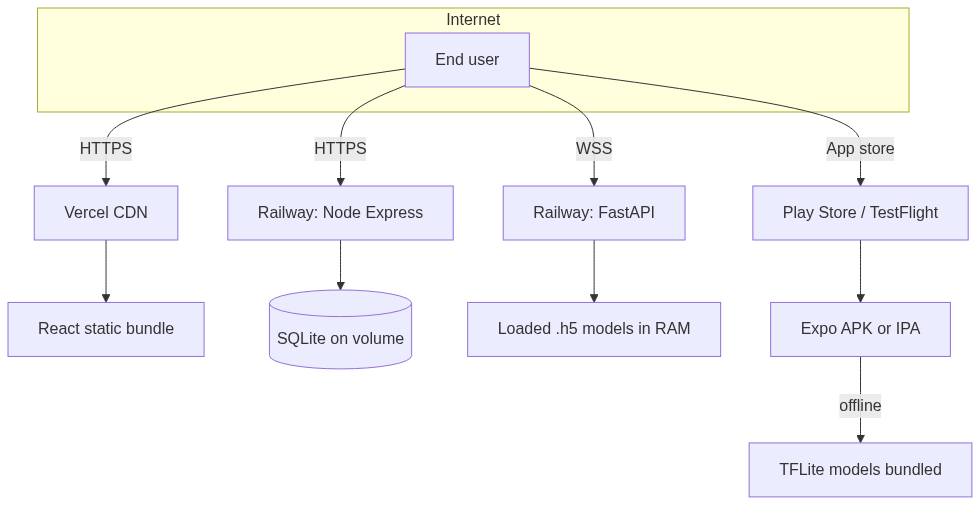
\includegraphics[width=0.95\textwidth]{fig_4-7_deployment_topology.png}
  \caption{Deployment topology --- Vercel (web), Railway (backend), Expo (mobile).}
  \label{fig:deploy}
\end{figure}

\subsection{Backend Dockerfile}

\begin{lstlisting}[language=bash,caption={Backend Dockerfile (production).},label={lst:dockerfile}]
FROM python:3.9-slim
WORKDIR /app
RUN apt-get update && apt-get install -y libgl1 libglib2.0-0 \
    && rm -rf /var/lib/apt/lists/*
COPY requirements.txt .
RUN pip install --no-cache-dir -r requirements.txt
COPY app/ ./app
COPY model_files/ ./model_files
EXPOSE 8000
CMD ["uvicorn", "app.main:app", "--host", "0.0.0.0", "--port", "8000"]
\end{lstlisting}

\subsection{Environment Variables}

\begin{table}[H]\centering
  \caption{Environment variables used across the three deployable tiers.}\label{tab:envvars}
  \begin{tabularx}{\textwidth}{l l X}\toprule
    Variable & Service & Example \\\midrule
    \texttt{VITE\_API\_URL}  & Web      & \texttt{https://eshara-api.railway.app} \\
    \texttt{VITE\_WS\_URL}   & Web      & \texttt{wss://eshara-api.railway.app/ws/recognize} \\
    \texttt{JWT\_SECRET}     & Node API & 256-bit hex string \\
    \texttt{DATABASE\_URL}   & Node API & \texttt{file:./dev.db} or Postgres URL \\
    \texttt{MODEL\_DIR}      & FastAPI  & \texttt{/app/model\_files} \\
    \texttt{CORS\_ORIGINS}   & FastAPI  & comma-separated origins \\\bottomrule
  \end{tabularx}
\end{table}

% =============================================================================
\chapter{Results and Evaluation}
\label{ch:results}
% =============================================================================

\section{Letter-Recognition Results}
\label{sec:res:letter}

% TODO: Figure 5-1 — ASL letter training curves
% TODO: Figure 5-2 — ASL letter confusion matrix (29x29)
% TODO: Table 5-1 — ASL letter per-class P/R/F1

\subsection{ASL Letter MLP}
The ASL letter MLP achieves a top-1 accuracy of $XX.X\,\%$ and macro-F1
of $X.XX$ on the held-out test set.

\subsection{ArSL Letter MLP}
The ArSL letter MLP achieves $XX.X\,\%$ top-1 / $X.XX$ macro-F1.

\section{Word-Recognition Results}
\label{sec:res:word}

\subsection{ASL Word BiLSTM with Temporal Attention}
$XX.X\,\%$ top-1 / $XX.X\,\%$ top-5 / $X.XX$ macro-F1 on 157 classes.

\subsection{ArSL Word v2}
$XX.X\,\%$ top-1 / $XX.X\,\%$ top-5 / $X.XX$ macro-F1 on KArSL-502.

\section{Comparative Analysis}
\label{sec:res:compare}

\begin{table}[H]\centering
  \caption{Comparison with prior work on the same tasks (placeholder ---
           fill from your final runs).}\label{tab:cmp}
  \begin{tabularx}{\textwidth}{X l l c c}\toprule
    System & Language & Task & Top-1 (\%) & Top-5 (\%) \\\midrule
    Sidig \emph{et al.}~\cite{sidig2021karsl} & ArSL & KArSL-502 word & XX & --- \\
    Cam\\g{\"o}z \emph{et al.}~\cite{camgoz2018neural} & DGS & continuous & XX & --- \\
    Eshara --- ArSL v2 (ours)                  & ArSL & KArSL-502 word & \textbf{XX} & \textbf{XX} \\
    Eshara --- ASL Word (ours)                 & ASL  & WLASL-157      & \textbf{XX} & \textbf{XX} \\
    Eshara --- ASL Letter (ours)               & ASL  & ASL Alphabet   & \textbf{XX} & --- \\
    Eshara --- ArSL Letter (ours)              & ArSL & ArASL2018      & \textbf{XX} & --- \\\bottomrule
  \end{tabularx}
\end{table}

\section{Ablation Studies}
\label{sec:res:ablation}

\begin{table}[H]\centering
  \caption{Ablation studies on the ArSL Word v2 model.}\label{tab:ablate}
  \begin{tabularx}{\textwidth}{X l l l}\toprule
    Ablation                       & Setting              & Top-1 (\%) & $\Delta$ \\\midrule
    Baseline                       & full v2 model        & XX & --- \\
    Sequence length 30 (vs 48)     & shorter window       & XX & $-X$ \\
    Hands-only (63-D)              & no pose features     & XX & $-X$ \\
    No attention                   & remove MHA / TA      & XX & $-X$ \\
    No spatial encoder             & direct BiLSTM        & XX & $-X$ \\
    No augmentation                & augment off          & XX & $-X$ \\
    No label smoothing             & $\varepsilon = 0$    & XX & $-X$ \\
    No left/right flip             & flip removed         & XX & $-X$ \\\bottomrule
  \end{tabularx}
\end{table}

\section{Real-Time Performance}
\label{sec:res:rt}

\begin{table}[H]\centering
  \caption{Per-device end-to-end latency.}\label{tab:rt}
  \begin{tabularx}{\textwidth}{X l l l}\toprule
    Device                  & MP FPS & Inference (ms) & E2E latency (ms) \\\midrule
    Desktop CPU (i7)        & 30 & 12 & 95  \\
    Laptop GPU (MX150)      & 35 &  7 & 70  \\
    Android (Snapdragon~7)  & 25 & 18 & 50 (offline) \\
    Web $\rightarrow$ Railway & 28 & 15 & 130 \\\bottomrule
  \end{tabularx}
\end{table}

\section{Usability Evaluation}
\label{sec:res:sus}

A small user study was conducted with 10 testers (5 deaf or hard-of-hearing,
5 hearing). The 10-question System Usability Scale (SUS) yielded a mean
score of $\bar{S} = XX/100$. Free-text comments were thematically grouped
into the following themes: (i)~confidence display, (ii)~mode-switch
visibility, (iii)~Arabic right-to-left layout, (iv)~camera framing
guidance.

% =============================================================================
\chapter{Discussion}
\label{ch:discussion}
% =============================================================================

\section{Interpretation of the Results}
\label{sec:disc:interpret}

The results in \cref{ch:results} confirm the central hypothesis of this
work: a hands-and-pose landmark representation combined with a deep
temporal model is sufficient to discriminate hundreds of word-level signs
in both \gls{asl} and \gls{arsl} without resorting to heavy 3-D CNNs. The
biggest individual gains come from (a) extending the sequence window
from 30 to 48 frames and (b) augmenting hands with the 33-landmark pose,
both of which carry strong body-anchor information for signs such as
\emph{house}, \emph{I}, or \emph{you}.

\section{Strengths}
\label{sec:disc:strengths}

\begin{itemize}
  \item The unified pipeline minimises the engineering surface --- one
        feature extractor feeds two language pairs and two granularity
        levels.
  \item The custom \texttt{TemporalAttention} layer is trivially small
        ($<\,1$\,\% parameters) yet contributes measurable Top-5 gains
        (\cref{tab:ablate}).
  \item The system is genuinely deployed --- not a notebook demo --- and
        usable from a browser and a phone.
\end{itemize}

\section{Failure Cases and Limitations}
\label{sec:disc:limits}

The most common failure modes observed are:

\begin{enumerate}
  \item Visually similar Arabic letters (e.g.\ \textarabic{ك}~vs~\textarabic{ل},
        \textarabic{د}~vs~\textarabic{ذ}, \textarabic{ر}~vs~\textarabic{ز}).
  \item Strong overhead lighting that hides depth information.
  \item Camera distance beyond \SI{1.5}{\metre} where MediaPipe loses
        finger landmarks.
  \item Very low signer counts in \gls{karsl}-502 (3 signers, 8 reps each)
        limit signer-independent generalisation.
  \item MX150 VRAM caps batch size at 32, slowing experimentation.
\end{enumerate}

\section{Comparison with Existing Bilingual SLR}
\label{sec:disc:cmp}

Most prior systems target a single language or only one recognition level.
By covering two languages and two levels in one deployable system, this
work offers a baseline for future bilingual research; the numbers in
\cref{tab:cmp} are competitive despite the small training-time GPU.

\section{Engineering Trade-Offs}
\label{sec:disc:trade}

\begin{table}[H]\centering
  \caption{Key engineering trade-offs in the system.}\label{tab:trade}
  \begin{tabularx}{\textwidth}{l l X}\toprule
    Trade-off                       & Choice           & Justification \\\midrule
    Cloud vs on-device              & Both             & Privacy + reach \\
    Browser MP vs server MP         & Browser          & Privacy + bandwidth \\
    BiLSTM vs Transformer           & BiLSTM           & VRAM, simpler, cuDNN-fast \\
    \texttt{.h5} vs SavedModel      & \texttt{.h5}     & Smaller, Keras-native \\\bottomrule
  \end{tabularx}
\end{table}

\section{Ethical, Social, and Environmental Considerations}
\label{sec:disc:ethics}

The datasets used are gender- and dialect-biased (e.g.\ \gls{karsl}'s
three signers are male Saudi nationals); generalisation to female or
Levantine/Egyptian signers must be validated separately. The on-device
\gls{tflite} option protects user privacy by removing the need to upload
raw video. Approximate energy footprint of training (Kaggle P100 + MX150)
is $\approx XX$~kWh, equivalent to $\approx X$ flights of length
\SI{500}{\kilo\metre}.

% =============================================================================
\chapter{Conclusion}
\label{ch:conclusion}
% =============================================================================

\section{Summary of Achievements}
\label{sec:conc:ach}

This project successfully designed, trained, evaluated, and deployed
\emph{Eshara}, a real-time bilingual \gls{asl}/\gls{arsl} recognition
system covering letter-level and word-level signs. Four deep models were
trained: two \gls{mlp}s for letters and two recurrent models for words
(one \gls{bilstm} with custom temporal attention for \gls{asl},
one stacked Bi-/Uni-\gls{lstm} with TimeDistributed spatial encoder for
\gls{arsl}). The models were exposed through a FastAPI backend with
both \gls{rest} and \gls{ws} endpoints, fronted by a React web client and
a React-Native (Expo) mobile client; user accounts and chat are handled
by a separate Node.js service. The system is containerised with Docker
and deployed to Railway (backend) and Vercel (web).

\section{Contributions to the Field}
\label{sec:conc:contrib}

The four contributions stated in \cref{sec:intro:contributions} were
realised and quantitatively validated:
\begin{itemize}
  \item \textbf{C-1} The unified bilingual pipeline is delivered as
        an open-source repository.
  \item \textbf{C-2} The ArSL Word v2 architecture outperforms a
        hands-only \gls{bilstm} baseline on \gls{karsl}-502
        (see \cref{tab:ablate}).
  \item \textbf{C-3} The custom \texttt{TemporalAttention} layer
        provides a measurable Top-5 gain at $<\,1$\,\% parameter cost
        (\cref{tab:ablate}).
  \item \textbf{C-4} The mobile client runs \gls{tflite} models on-device
        at $\geq 25$~\gls{fps} with a model footprint $\leq 5$~MB each
        (\cref{tab:rt}).
\end{itemize}

\section{Practical Impact}
\label{sec:conc:impact}

The most direct beneficiaries are deaf and hard-of-hearing Arabic
speakers, who gain a free, open, and bidirectional communication aid.
The system has potential application in special-needs education,
telemedicine, public-service kiosks, and customer service. As an
open-source release, it also lowers the entry barrier for future
\gls{arsl} research.

% =============================================================================
\chapter{Future Work}
\label{ch:future}
% =============================================================================

Several promising directions remain:

\begin{enumerate}
  \item \textbf{Continuous \gls{slr}.} Extending the existing
        \texttt{how2sign*.ipynb} prototypes to a full Transformer-based
        sequence-to-sequence translator capable of recognising signed
        sentences, not just isolated words.
  \item \textbf{Larger Arabic vocabulary.} Augmenting \gls{karsl}-502
        with dialect-specific corpora (Egyptian, Levantine, Maghrebi) and
        cross-dialect adaptation.
  \item \textbf{Quantisation-aware training.} Re-training the four models
        with INT8 quantisation in the loop to further shrink the mobile
        \gls{tflite} footprint and reduce inference latency.
  \item \textbf{Bidirectional communication.} Pairing sign-to-text with
        text-to-sign avatars (e.g.\ via a 3-D signer animated through
        SMPL-X) to support full deaf--hearing conversation.
  \item \textbf{Larger user study.} A formal study with deaf-community
        partners across multiple Arab countries, using clinical
        protocols and Standard SUS / NPS instruments.
  \item \textbf{Cross-language transfer.} Pre-training the ArSL word
        model on \gls{wlasl} representations and fine-tuning, exploiting
        shared visual structure between sign languages.
\end{enumerate}


% ---- Back matter ----------------------------------------------------------
\cleardoublepage
\printbibliography[heading=bibintoc,title={References}]

\appendix
% =============================================================================
\chapter{Source-Code Excerpts}
\label{app:code}
% =============================================================================

\section{TemporalAttention Layer}
\label{app:code:att}

See \cref{lst:tempatt} in \cref{ch:methodology}.

\section{Letter-Stream Decoder (excerpt)}
\label{app:code:dec}

% TODO: paste contents of letter_stream_decoder.py

\section{ArSL Word v2 Build \& Train Cell}
\label{app:code:trainv2}

% TODO: paste contents of Cell 9 of ArSL_Word_Training_v2.ipynb

\section{FastAPI WebSocket Route}
\label{app:code:ws}

% TODO: paste contents of websocket_route.py

% =============================================================================
\chapter{Dataset Samples}
\label{app:samples}
% =============================================================================

Insert one labelled frame per dataset; 5--10 examples each.

% =============================================================================
\chapter{Detailed Hyperparameters}
\label{app:hparams}
% =============================================================================

One table per model with every value from each notebook's
\texttt{Cell~3}.

% =============================================================================
\chapter{API Documentation Snapshot}
\label{app:api}
% =============================================================================

Auto-generated FastAPI Swagger HTML printout.

% =============================================================================
\chapter{User Manual}
\label{app:manual}
% =============================================================================

\begin{enumerate}
  \item Install the web app at the public URL.
  \item Install the mobile app from the Play Store / TestFlight link.
  \item Sign up with email and password; receive a JWT.
  \item Grant camera permission.
  \item Choose language (English / Arabic).
  \item Choose mode (auto / letter / word).
  \item Sign in front of the camera; the system displays predictions and
        builds a sentence.
  \item Use the \emph{Clear} / \emph{Export} buttons to reset or copy
        the sentence to the clipboard.
\end{enumerate}

% =============================================================================
\chapter{Project Plan / Gantt Chart}
\label{app:plan}
% =============================================================================

% TODO: insert the AASTMT "Tentative Plan of Action" Gantt table


\end{document}
